\documentclass[a4paper,10pt]{scrartcl}
\usepackage[T1]{fontenc}
\usepackage[utf8]{inputenc}
\usepackage[style=ieee,backend=biber,maxbibnames=9,sorting=anyt,sortcites=true,citestyle=numeric]{biblatex}
\usepackage{amsmath,amsfonts}
\usepackage{scrpage2}
\usepackage{scrtime}
\usepackage{setspace}
\usepackage{enumerate}
\usepackage{enumitem}
\usepackage{graphicx}
\usepackage{caption}
\usepackage{subcaption}
\usepackage{multirow}
\usepackage{verbatim}
\usepackage{color}
\usepackage{url}
\definecolor{InnerLinkColor}{rgb}{0.208,0.374,0.486}
\definecolor{OuterLinkColor}{rgb}{0.216,0.439,0.388}
\usepackage[colorlinks,breaklinks,
linkcolor=InnerLinkColor,filecolor=OuterLinkColor,
menucolor=OuterLinkColor,urlcolor=OuterLinkColor,
citecolor=InnerLinkColor]{hyperref}
\usepackage[paper=a4paper,left=25mm,right=25mm,top=20mm,bottom=25mm]{geometry} 

\newcommand{\tab}[1]{\hspace{.1\textwidth}\rlap{#1}}

\title{Network Function Forwarding Graph API documentation}

\author{Bal\'azs N\'emeth, J\'anos Czentye, Bal\'azs Sonkoly\\
  Budapest University of Technology and Economics (BME)\\
  \{balazs.nemeth,janos.czentye,balazs.sonkoly\}@tmit.bme.hu}

\begin{document}

\maketitle

\section*{About this document}

This document was created as a help to understand the the main concepts of NFFG library of ESCAPEv2 and 
to use its provided API for orchestration purposes.
The code was written by BME and published at \url{https://gitlab.fp7-unify.eu/Balazs.Sonkoly/escape-shared}, 
a generated documentation and installation instructions for ESCAPEv2 and other information are available at
 \url{https://sb.tmit.bme.hu/escape/}, 
 which documentation contains far more classes and functions that are needed for 
 acquiring sufficient information for the orchestration, thereafter it is referred to by \emph{generated documentation}.
 The reader is assumed to have an idea about the main principles of the multi-layered Unify architecture.

\section{Service Graph Embedding problem}

The Service Graph Embedding (SGE) problem is rooted in the well-studied Virtual Network Embedding (VNE) problem.
The reader is assumed to be familiar with VNE and the according research approaches. 
SGE is about embedding multiple Service Graphs (SG) onto a shared Resource Graph (RG) 
representing the physical/virtual resources of the infrastructure (also called substrate in the present document).

Network Functions (NF) in SG must be mapped to the hosts of RG, for which collocation 
(the placement of two NFs to the same host) must be allowed. 
Links of the SG must be mapped to simple paths of the RG, in a way the logical connections represented 
by the links of the SG must be held after the NF mapping to hosts.
Furthermore, all requirements (described later) must be strictly respected.

The most important difference from VNE is the consideration of end-to-end requirements in the SG.
For this purpose nodes of both graphs are separated into three groups:
\begin{itemize}
\item NFs - describing the service components - in SG
\item hosts - providing the computation capacity - in RG
\item Service Attachment Points (SAP) - defining the endpoints in both graphs
\end{itemize}
This way, end-to-end paths are considered as a simple path between two SAP nodes. 

An illustrative example is presented in \ref{sge}, where NFs are pictured with blue rectangles denoted as $nfX$ in the SG,
 hosts are green rectangles denoted as $hostX$ and SAPs are ovals denoted as $sapX$ in both graphs. 
SG links are pictured by continuous arrows in the SG, and numbered incrementally.
Two end-to-end paths are selected between $sap1-sap2$ and $sap1-sap3$. 
These paths can share SG links and NFs with each other as it is shown by SG link $\#1$ and $nf1$.
There can be parallel SG links (e.g. $\#3, \#4$) and links which are not in any end-to-end paths (e.g. $\#7$).

\begin{figure}
\centering
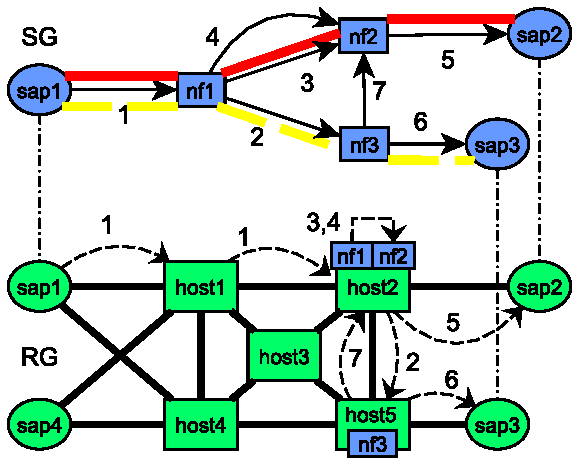
\includegraphics[scale=1.0]{SGE}
\caption{Illustrative example for Service Graph Embedding}
\label{sge}
\end{figure}

The following list gives some further details on the parameters.

\subparagraph{Resource Graph:}
\begin{itemize}
\item Arbitrary directed (there can be parallel edges, loops),
\item Host node attributes: 
	\begin{itemize}
	\item forwarding bandwidth (sum of bandwidths between all ports - cumulative bandwidth, or switching capacity)
	\item guaranteed latency between any ports (independent of traffic load)
	\item set of runnable NF types (set of literals)
	\item CPU, memory, storage resources
	\end{itemize}
\item SAP nodes:
	\begin{itemize}
	\item They can be mapped unambiguously by their ID-s, which is the same in both graphs, there are no other mapping constraints on them.
	\end{itemize}
\item Link attributes:
\begin{itemize}
	\item bandwidth
	\item latency (independent of traffic load)
\end{itemize}
\end{itemize}

\subparagraph{Service Graph:}
\begin{itemize}
\item Arbitrary directed (no need for connectedness, nor DAG, nor simpleness),
\item NF instance attributes:
	\begin{itemize}	
	\item NF type of the NF instance
	\item CPU, memory, storage requirement
	\end{itemize}
\item SAP nodes:
	\begin{itemize}	
	\item same as in the Resource Graph
	\end{itemize}
\item Link attributes:
	\begin{itemize}	
	\item bandwidth requirement
	\item latency requirement
	\item flowclass (to differentiate traffic if there is a decision point)
	\end{itemize}
\end{itemize}

\subparagraph{Service Chains (end-to-end requirements):}
\begin{itemize}
\item Requirement applied to a single, loopless path, without branches, starting from a SAP and ending in a SAP (ending and starting SAPs can be the same):
\item Sequence of NF instances from Service Graph
\item Sequence of Service Graph links (choosing one of the parrallel links, in case NF instance list is not enough to specify it), these together specify the path for the end-to-end requirement.
\item Maximal allowed latency on the path
\item Minimal required bandwidth on the path
\end{itemize}

\section{NFFG in general}

The Network Function Forwarding Graph structure is intended to provide a joint abstraction for 
$(a)$ computing and networking resources (RG definition); 
$(b)$ service and quality of service requirement description (SG definition); and 
$(c)$  mapping of SG elements to RG elements according to the SGE problem definition. 

The notation $\mathcal{S}(NFFG)$ represents the set of structures which complies to the definition of NFFG format.
Generally, an orchestration algorithm shall implement the following function:

$$ Orchestrate: \mathcal{S}(NFFG) \times \mathcal{S}(NFFG) \rightarrow \mathcal{S}(NFFG) $$
and
$$ req, net, map \in \mathcal{S}(NFFG): Orchestrate (req, net) = map $$
where $map$ solves the SGE problem defined by $req$ and $net$, and minimizes the resource utilization defined by $map$.

\subsection{Service Graph mapper}

An illustrative example of an orchestration scenario is shown in \ref{fig:nffg-illustration}. 

The service requirement comes as the SG from the northbound interface of the architecture, 
this graph complies to the NFFG structure (but does not contain any resource nodes). 
An end-to-end requirement is given by EdgeReq between $SAP0$ and $SAP1$, and the chosen path is $SAP0-NF1-NF3-SAP1$.

A simple RG is presented by the Resource Orchestration layer, aggregating all of its resources to a single node
\footnote{This is called the Single BigSwitch-BigSoftware abstraction model, 
where a whole (part of a) network is aggregated into a single node.}, providing a virtualized view of the network,
which complies to the NFFG format (even though it does not contain any NF).

The SG mapper calculates a trivial mapping between the virtualized resource and the service description,
and produces an output in NFFG format (called $NFFG$ in \ref{fig:nffg-illustration}). 
The SAP nodes are mapped unambiguously to their counterparts in the RG.
A set of abstract flowrules describe the appropriate forwarding information in $node0$, 
preserving the semantic meaning specified by the SG.

\subsection{Resource Orchestration}

The Resource Orchestration (RO) layer receives the service description in NFFG format 
(graph $NFFG$ in \ref{fig:nffg-illustration}),
which can contain substrate nodes (e.g. $node0$ in \ref{fig:nffg-illustration}).
A RG is received from the southbound interface of the architecture, 
jointly specifying the network and compute resources, which also complies to the NFFG format
\footnote{Any of these RG nodes (e.g. $node12$ in \ref{fig:nffg-illustration}) 
can cover (virtualize) a part of the network and have inner orchestration.}.

The Network Function Information Base (NFIB) contains information about the NFs, 
such as resource requirements, deployment information, equivalent decomposition into a graph of NFs, etc., 
(Note: currently these features are not integrated into the orchestration function, 
every information what shall be used for orchestration can be gathered from the NFFG describing the service.)

After the resource orchestration finished and all EdgeSGLinks are mapped to a path in the RG 
and all NFs have a place where they can be executed satisfying all the end-to-end and local requirements,
The RO should produce the output NFFG, indicating the decisions of the orchestration function by 
connecting the NFs to their hosts, and installing the abstract flowrules to steer the traffic between 
appropriate NFs according to the EdgeSGLinks. It is illustrated by the graph of $NFFG$ in \ref{fig:nffg-illustration},
which should be the final output of the orchestration algorithm.

(Note: In a recursive orchestration scenario, when the nodes of the RG can have inner orchestrators, 
a splitting of EdgeReqs shall be calculated in addition to the previously explained output. 
In this case loop EdgeReqs shall be drawn between the appropriate ports of a resource node, 
defining the required end-to-end requirement in the virtualized domain. 
Every aspect of the orchestration function can be examined without this feature.)

\begin{figure}[ht!]
  \centering
  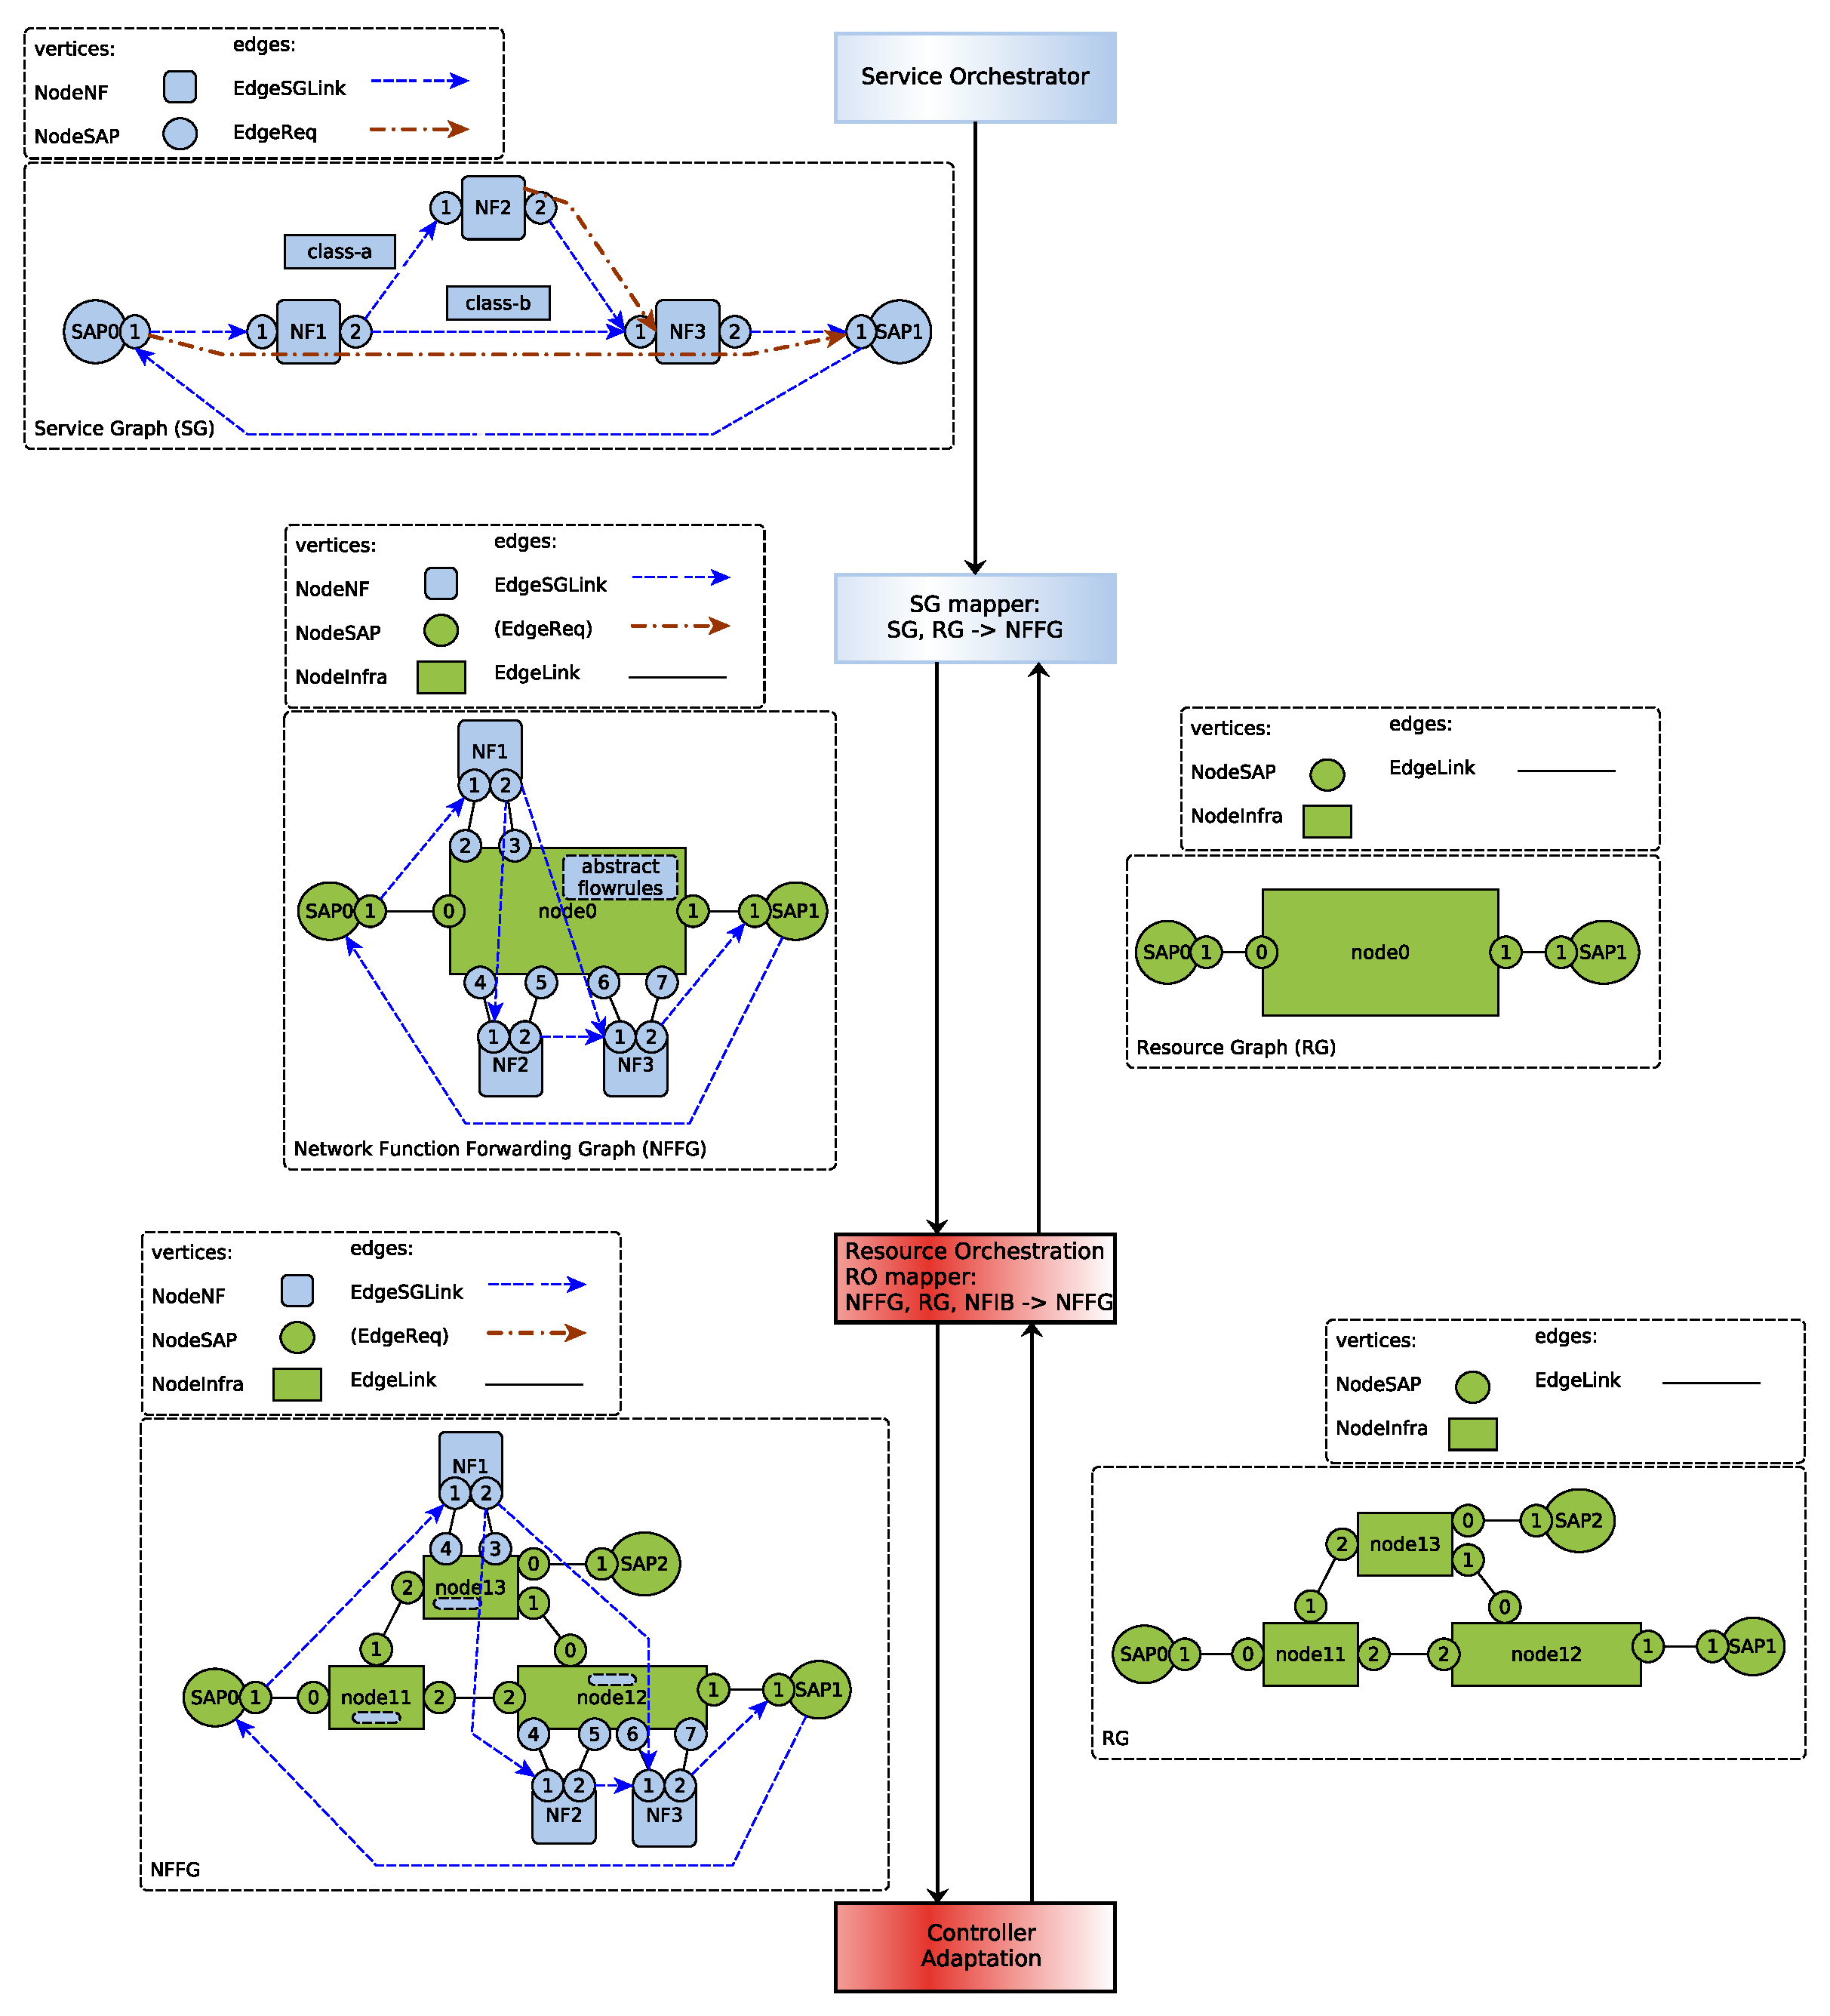
\includegraphics[width=\textwidth]{NFFG-illustration}
  \caption{Illustration of SG, RG, and NFFG}
  \label{fig:nffg-illustration}
\end{figure}


\section{NFFG API documentation}

The Python implementation of the NFFG library can be found in the repository 
\emph{escape-shared / escape / escape / nffg\_lib} folder. 
The NFFG is a wrapper around a NetworkX \footnote{https://networkx.github.io/} graph library, so an NFFG structure is a single Python object providing different node and link types and extra features for the NetworkX graph. 
Sometimes a class attribute is implemented by a built-in Python type (e.g. container implemented as a list), 
in this case they are referred to as "built-in". 
Inheritance relationship between two classes are noted by \emph{BASECLASS} in the class description,
this means the class which has a BASECLASS, have every attribute as its base, 
and only the additional attributes are described.

The NFFG library consists of two files:
\begin{itemize}
\item nffg\_elements: implementation of link and node types, and their features
\item nffg: implementation of structure construction, modification and information retrieval
\end{itemize}

The NFFG structure can be saved to a JSON formatted file with all of its data, 
and later it can be read again to create an equivalent NFFG object. 
This can be done with \emph{dump()} and \emph{parse()} functions of the NFFG object.

\subsection{NFFG elements}

\subparagraph{Flowrule}
Abstract flowrule representation. Flowrules are stored in Port objects, 
they have an OpenFlow-like format for the match and action fields, 
but these are not needed to be accessed directly for orchestration purposes.
They store how much bandwidth are occupied for them. Flowrules are stored in InfraPort 
objects, where they originate from (so in\_port's argument is always the containing port's ID).
\begin{itemize}
\item hop\_id - Which EdgeSGLink instance's path does this flowrule belong to
\item bandwidth - The EdgeSGLink's bandwidth requirement
\item latency - The EdgeSGLink's latency requirement
\item match - Possible values separated by semicolons (;): "in\_port=<<Port.id>>", 
"TAG=<<TAG name to match for>>", "flowclass=<<flowtype,e.g.:HTTP>>". All of these are 
concatenated together into one string.
\item action - Possible values separated by semicolons (;): "output=<<Port.id>>", 
"TAG=<<TAG name to put on>>", "UNTAG". All of these are concatenated together into one string.
\end{itemize}

\subparagraph{Port}
Represents a port of Node. Belongs to exactly one Node object. 
\begin{itemize}
\item id - Globally unique identifier
\item node - The containing Node object can be accessed through this variable
\end{itemize}

\subparagraph{InfraPort}
Represents a port of an NodeInfra. Belongs to exactly one NodeInfra. 
Used to store Flowrule objects, flowrules can only be stored in InfraPort objects.
\begin{itemize}
\item BASECLASS: Port
\item flowrules - Built-in list of Flowrule objects contained in this InfraPort.
\end{itemize}

\subsubsection{Node types}

\subparagraph{Node}
Base class for all node objects, \emph{cannot be in the NFFG structure}, collects base functionalities.
\begin{itemize}
\item id - Globally unique identifier (also used as id in the NetworkX object)
\item name - Globally unique readable name, should be used for graphical representation
\item NF, INFRA, SAP - Defined constants strings (three separate attributes)
\item type - Defines what type of node is this object, one of \{Node.NF, Node.INFRA, Node.SAP\} constants
\item ports - Container for the Port objects of the Node, 
Port objects with "id" can be accessed as Node.ports[id], iterable, 
inclusion can be tested, length can be access using built-in $len()$. 
NodeNFs have Port classes as their port object, while NodeInfras have InfraPorts as their port object.
\end{itemize}

\subparagraph{NodeResource}
Stores the resources associated with a node (as requirement or resource). 
The units of the components are not fixed, they are all real numbers. 
The units advised to be used are noted for every components.
Attributes can be set or read as if the NodeResource object would be a built-in Python dictionary 
(e.g. NodeResource['cpu'] = 5).
\begin{itemize}
\item cpu - Number of CPU cores / abstract computation metric.
\item mem - Memory of the node (MB)
\item storage - Storage of the node (GB)
\item delay - Delay of the node  (to be specified later) (ms)
\item bandwidth - Bandwidth of the node (to be specified later) (Mb/s)
\end{itemize}

\subparagraph{NodeNF}
Network Function instance node of the NFFG. Abstractly represents some basic network functionality 
implemented by a virtual machine, legacy hardware, Click process, etc. All ports are objects with type of Port.
\begin{itemize}
\item BASECLASS: Node
\item functional\_type - The type of the NodeNF referring to its implemented functionality, 
stored as a string literal (e.g. headerCompressor).
\item res - NodeResource object defining the resource requirement of the NodeNF instance. 
The \emph{delay} and \emph{bandwidth} parameter is unused so far, 
can gain meaning after the adoption of NF decomposition to the orchestration.
\end{itemize}

\subparagraph{NodeInfra}
Computation and/or forwarding node of the NFFG. All ports are objects with type of InfraPort, 
where Flowrule objects can be stored.
\begin{itemize}
%\item (TODO: Recursive orchestration support, end-to-end delay requirement splitting, infra\_type field are omitted!!ok?)
\item BASECLASS: Node
\item supported - Built-in list of literals of the supported NF functional types.
\item res - Provided maximal resources stored in NodeResource object which is provided 
if the NodeInfra is completely unloaded. The cpu, mem, storage and bandwidth parameters are additively decreased 
if the NodeInfra is loaded by NodeNFs, but latency is independent of network or computation load. 
Delay parameter is the value which is guaranteed between all of the port pairs of the NodeInfra.
Bandwidth parameter is considered as switching capacity, in other words, 
the sum of the bandwidth of all the traffic forwarded between any port pairs cannot exceed this value.
\end{itemize}

\subparagraph{NodeSAP}
Class for representing the endpoint in the NFFG. During the orchestration process 
the mapping of NodeSAPs of the NFFG defining the SG, shall be unambiguous by determining 
the NodeSAP object in the NFFG of the RG with the same id attribute. 
\begin{itemize}
\item BASECLASS: Node
\end{itemize}

\subsubsection{Link types}

\subparagraph{Link}
Base class for all edge classes of NFFG. \emph{Cannot be present in the NFFG.}
\begin{itemize}
\item src - Source Port object of the link
\item dst - Destination Port object of the link
\item id - Globally unique identifier (also used in NetworkX as the key for the parallel edges between two nodes)
\item STATIC, DYNAMIC, SG, REQUIREMENT - Defined constant strings (four separate attributes)
\item type - Defines what kind of object is this link, one of \{Link.STATIC, Link.DYNAMIC, Link.SG, Link.REQUIREMENT\}
\end{itemize}

\subparagraph{EdgeLink}
Class for infrastructure links in the NFFG structure if its type is Link.STATIC. 
\begin{itemize}
\item BASECLASS: Link
\item type - Can only be Link.STATIC or Link.DYNAMIC. STATIC links can only be between substrate nodes or SAPs, 
indicating data transfer capability between the substrate elements (describing actual Resource Graph topology).
DYNAMIC links can only be between NodeNF and NodeInfra type objects. 
The role of DYNAMIC links is to indicate mapping relation between a NF and a substrate node. 
Mapping relation must be made bidirectional by adding a DYNAMIC link in both directions.
\footnote{DYNAMIC links do NOT indicate substrate connection, so logical links of the SG must not be mapped to these links, 
and they shall be ignored during path calculation, out-edge degree of a substrate node, etc.}
If a NodeNF has multiple ports, one separate DYNAMIC EdgeLink object exists for each of them, 
connecting the NodeNF to a single NodeInfra, ending in separate InfraPort objects of the hosting NodeInfra.
\item delay - Forwarding delay of the substrate link (If the link is DYNAMIC, this field is ignored). 
\item bandwidth - Maximal available bandwidth capacity of the substrate link (If the link is DYNAMIC, this field is ignored).
\end{itemize}

\subparagraph{EdgeSGLink}
Class for logical connections between NodeNFs. Can only exist between NodeNFs or SAPs.
This class is used to describe the SG and its SG-link-local resource requirements.
\begin{itemize}
\item BASECLASS: Link
\item delay - The maximal allowed latency between the two NodeNFs which are connected by this EdgeSGLink object.
\item bandwidth - The minimal required bandwidth between the two NodeNFs which are connected by this EdgeSGLink object.
\item flowclass - Defines a filter for a subset of the traffic 
\footnote{e.g. two SG links start from the same port of the same NodeNF (otherwise the NodeNF knows the role of the ports)
and one of  them is applied to HTTP traffic, while the other is to non-HTTP traffic. 
This example is illustrated in the SG of \ref{fig:nffg-illustration}, where two EdgeSGLinks start from port number 2 of NF1.}. 
Probably not needed for orchestration itself.
\end{itemize}

\subparagraph{EdgeReq}
Class for defining end-to-end requirements between SAP nodes. Can only be between NodeSAP objects.
They shall be ignored in the NFFG of RG.
\begin{itemize}
\item BASECLASS: Link
\item sg\_path - Selects a simple directed path between the source and destination NodeSAP objects. 
Can only select from the EdgeSGLink objects of the NFFG of the SG, 
and refers to them by their unique identifier (Link.id attribute).
Implemented by a built-in list (which has predictable iteration order). 
The following required end-to-end QoS parameters must be satisfied on the RG path where these
(sequence of) SG links will be mapped.
\item delay - The required maximal latency on the defined SG path.
\item bandwidth - The required minimal bandwidth capacity on the defined SG path.
\end{itemize}

\subsection{Modification of NFFG}

All elements have addition and deletion functions, del\_* and add\_* respectively. 
The place of these functions are intuitive, 
e.g. NodeNF, EdgeReq addition can be called on NFFG objects, Port addition can be called on any node, etc.
The id of an element is always sufficient for a deletion function. 
Deleting a node will remove all the link which start or end in the deleted node.

For the description of element addition parameters consult the generated documentation; 
their usage is quite straightforward, and almost every parameter can be omitted and left default or unrestricted.
If a parameter is left undefined, the corresponding attribute is set to the built-in \emph{None}, 
which should be handled based on the type of the missing parameter (e.g. If a EdgeSGLink.delay is \emph{None}, 
the link requirement shall be assumed unrestricted or infinite required worst case latency).

\subparagraph{clear\_links}
Removes all the links of the given link type. Can be called on NFFG objects.

Parameters:
\begin{itemize}
\item link\_type - The defined link type, one of \{Link.STATIC, Link.DYNAMIC, Link.SG, Link.REQUIREMENT\}.
\end{itemize}

\subparagraph{clear\_nodes}
Removes all the nodes of the given type. Can be called on NFFG objects.

Parameters:
\begin{itemize}
\item node\_type - The defined node type, which all are intended to be removed, one of \{Node.NF, Node.INFRA, Node.SAP\}.
\end{itemize}

\subparagraph{add\_undirected\_link}
Adds a EdgeLink object between two nodes in both direction. Useful when one would like to add DYNAMIC link 
(mapping relation) between a NodeNF and a NodeInfra, because this connection must be bidirectional.

Parameters:
\begin{itemize}
\item port1 - One end of the links. This field must be given.
\item port2 - Other end of the links. This field must be given.
\item p1p2id - Value of Link.id field in one direction (optional).
\item p2p1id - Value of Link.id field in the other direction (optional).
\item dynamic - Boolean value, indicating whether this EdgeLink pair should be DYNAMIC or STATIC. Defaults to \emph{False}.
\item delay - Value of EdgeLink.delay.
\item bandwidth - Value of EdgeLink.bandwidth.
\end{itemize}

\subparagraph{copy}
Returns a full copy of the NFFG structure. Every object is duplicated, 
the returned new object will be independent of the previous one.

\subsection{Information about the NFFG}

\subsubsection{Directly available information}

The following paragraphs are all directly accessible attributes of an NFFG object.

\subparagraph{network}
The wrapped NetworkX object can be reached using the $network$ attribute of an NFFG object. 
Due to the different link and node types defined in NFFG, this object should be handled with care, 
because in the scope of NetworkX there only exist \emph{relation}s between \emph{node}s,
while in the NFFG structure these are differentiated by the types, 
providing different meaning for each node and link type. In other words, the wrapped NetworkX 
object is completely unaware of the different types of links and nodes and their meanings.
For example during the calculation of the degree count of an InfraNode all DYNAMIC and STATIC links
are considered, although only the STATIC links are actual infrastructure links.

\subparagraph{infras}
Iterator on all the NodeInfra objects of the NFFG structure. 

\subparagraph{saps}
Iterator on all the NodeSP objects of the NFFG structure. 

\subparagraph{nfs}
Iterator on all the NodeNF objects of the NFFG structure. 

\subparagraph{sg\_hops}
Iterator on all the EdgeSGLink objects of the NFFG structure. 

\subparagraph{links}
Iterator on all the EdgeLink (DYNAMIC \emph{OR} STATIC type) objects of the NFFG structure. 

\subparagraph{reqs}
Iterator on all the EdgeReq objects of the NFFG structure. 

\subparagraph{infra\_neighbors}
Returns an iterator on the NodeInfra objects of the NFFG structure which are neighbours to the given Node object.
Can be used on NodeNFs to determine where they are mapped. 
Can be used on NodeInfras to iterate on its substrate (NodeInfra) neighbours.

Parameters:
\begin{itemize}
\item node\_id - The unique identifier value (Node.id) of the node object whose neighbours shall be returned. 
\end{itemize}

\subparagraph{running\_nfs}
Returns an iterator on the NodeNF objects which are neighbouring (mapped) to the given NodeInfra object.

Parameters:
\begin{itemize}
\item infra\_id - The unique identifier value of a substrate node. Can only be NodeInfra.id value.
\end{itemize}
	
\subsubsection{Calculable information}

The resource parameters stored in the NFFG of a RG, are all considered to define the maximal available resource of RG.
As far as the NFFG also expresses the mapping of NodeNFs, 
their requirements shall be subtracted from the maximal resources to get the actual available resources, 
which are needed for orchestration purposes.

\subparagraph{calculate\_available\_link\_res}
Based on the Flowrule objects of the whole NFFG, the available bandwidth can be calculated by subtracting all the 
reserved bandwidth values for each Flowrule. Calculates bandwidths only for links, not nodes. 
Stores the currently available bandwidth value in a EdgeLink.availbandwidth attribute added to each object by this function.
This is a method of the NFFG class.

Parameters:
\begin{itemize}
\item sg\_hops\_to\_be\_ignored - A container for the set of EdgeSGLink.id-s whose flowrules (defining its path in the NFFG)
shall be ignored when subtracting the bandwidth resource from the maximal available bandwidth capacity.
\end{itemize}

\subparagraph{calculate\_available\_node\_res}
Calculates the available resources of the NodeInfras based on the resource requirements of the mapped NodeNFs. 
Also uses the Flowrules of the NodeInfras to calculate their available bandwidth capacities. 
Stores the calculated values in a NodeInfra.availres attribute, which is a NodeResource object.

Parameters:
\begin{itemize}
\item vnfs\_to\_be\_left\_in\_place - A dictionary of NodeNF-s, keyed by their NodeNF.id, and its data 
is the NodeNF object itself. These NodeNFs are ignored during the calculation of available resources, 
and the contained NodeNFs' NodeResource objects are updated in the NFFG. 
The parameter's default value is an built-in empty dictionary, which means no NodeNF is ignored.
Two NodeNF are considered to be identical if their ID-s are the same.
\end{itemize}

The available resource information is not persisted by the \emph{NFFG.dump()} function, 
so it cannot be retrieved by \emph{NFFG.parse()}. So after parsing an NFFG object, the calculable 
information shall be calculated again.

%TODO: Check some NFFG syntax info? (DYNAMICs are bi, no DYNAMIC betwwen NF and infra, no unnecesssary EdgeReq)

\section{Examples of NFFG API usage}

%% examples for 
%	calulate resources, 
%	purge RG and SG, 
%	identify graph connections one by one (iterate, link->port->node access)

\subsection*{Get all substrate connections of RG}

for link in nffg.links: 

if link.type == Link.STATIC:

There is a link between nodes $link.src.node$ and $link.dst.node$ objects.

\subsection*{Get the currently mapped NodeNFs}

for nf in nffg.running\_nfs(infra.id):

$nf$ is a NodeNF mapped to $infra$.

\subsection*{Delete all NodeNFs from the RG}

nffg.clear\_nodes(Node.NF)

\subsection*{Get currently available resources}

nffg.calculate\_available\_node\_res()

for infra in nffg.infras:

$infra$ has $infra.availres['cpu']$ available CPU capacity.

\subsection*{Get the path from SG which is referred by EdgeReq}

for edgesglink\_id in edgereq.sg\_path:

for edgesglink in nffg.sg\_hops:

if edgesglink.id == edgesglink\_id:

$edgesglink$ is a part of $edgereq$'s end-to-end path.

\end{document}
